% \documentclass[pdftex,12pt,a4paper]{report}
\documentclass[12pt,a4paper]{article}

\usepackage{anysize}
\marginsize{3cm}{3cm}{3cm}{3cm}
\usepackage{graphicx}
\usepackage{t1enc}
\usepackage[MeX]{polski}
\usepackage[utf-8]{inputenc}
\usepackage[T1]{fontenc}
\usepackage{subfigure}

\usepackage{fancyhdr}
\setlength{\headheight}{15pt}
\pagestyle{fancy}

\newcommand{\HRule}{\rule{\linewidth}{0.5mm}}

\begin{document}

\input{./tex/title.tex}

\fancyhf{}

\lhead{Tomasz Huczek, Andrzej Jasiński}
\rhead{\today}
\rfoot{\thepage}

\begin{abstract}
 Niniejsza dokumentacja dotyczy projektu wykonanego w ramach laboratorium z przedmiotu \textbf{Sprzęt Komputerowy Systemów Sterujących}. Projekt ma za zadanie zasymulować zjawiska zachodzące na stole bilardowym wzorując się na prawach fizyki, oraz wykorzystując możliwości współczesnych kart graficznych do zaprezentowania realnego, trójwymiorawego obrazu wysokiej jakości.
\end{abstract}


\tableofcontents
\newpage


\section{Wstęp}
Wykonanie realistycznej symulacji wiązało się z odpowiednim zamodelowaniem zjawisk fizycznych. W pierwszym rozdziale opisujemy w jaki sposób zasymulowaliśmy podstawowe prawa fizyki pozwalające na realistyczne zamodelowanie zjawisk zachodzących na stole bilardowym. W kolejnym rozdziale opisujemy jakich technik użyliśmy aby zaprezentować rezultat symulacji na ekranie. Rozdział opisuje w skrócie wykorzystane techniki renderingu przy użyciu biblioteki OpenGL oraz niskopoziomowe programowanie procesora grafiki przy użyciu techniki \textit{shaderów}.\\
Kolejne rozdziały opisują już działanie samego programu, jego obsługa raz testowanie.

\section{Fizyka}
\subsection{Zasady dynamiki Newtona}

Przyspieszenie bil, a co za tym idzie opis wektorowy trajektorii bil jest oparty na zasadach 
dynamiki Newtona, zgodnie z drugą zasadą:

\begin{equation}
\vec a = \frac{\vec F}{m}
\end{equation}



\subsection{Zasada zachowania pędu i energii}
\subsection{Kolizje}

\begin{figure}[h]
  \centering
  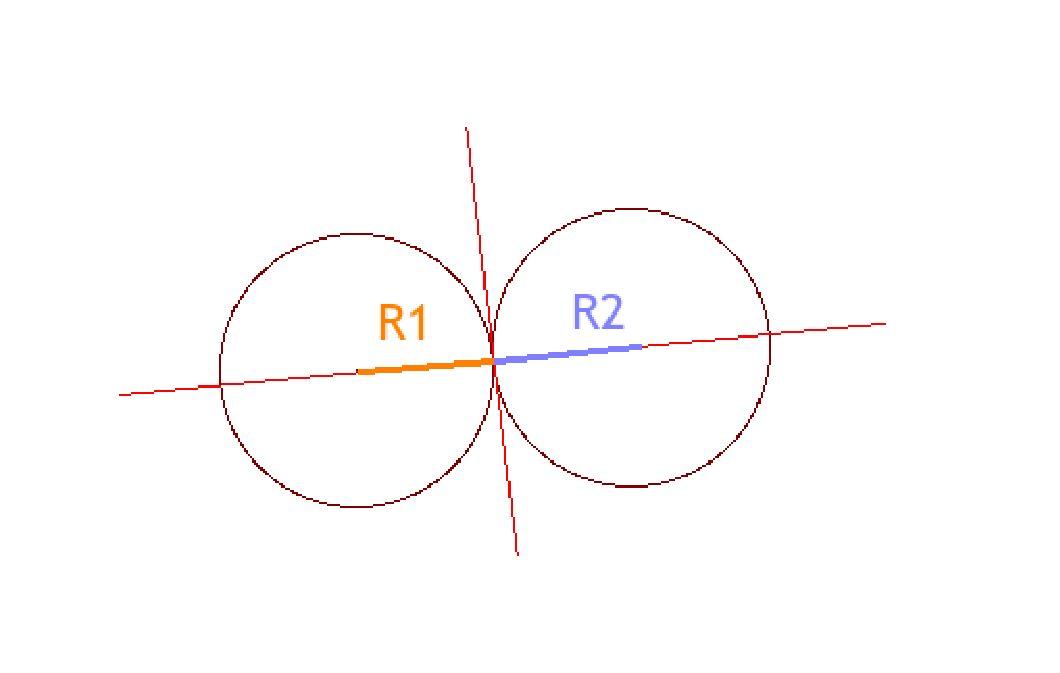
\includegraphics[width=0.5\textwidth]{./img/bb_col.eps}
  \caption{Kolizja bila - bila}
  \label{fig:bbcol}
\end{figure}

Kolizje obliczne są w możliwie najprostszy i najszybszy sposób. W naszej symulacji mamy dwa rodzaje kolizji:
\begin{itemize}
 \item bila - bila
 \item bila - banda
\end{itemize}

\begin{figure}[h]
  \centering
  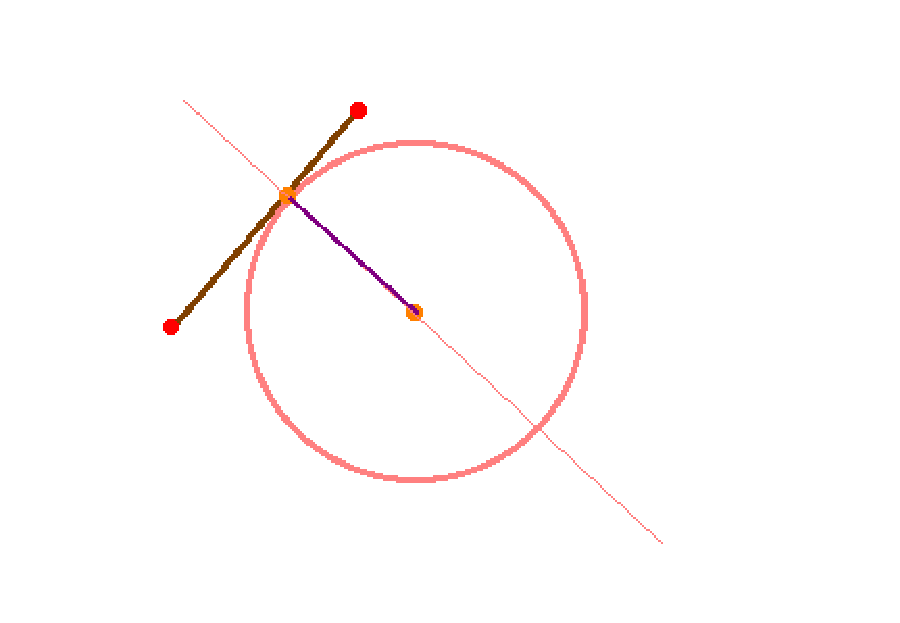
\includegraphics[width=0.5\textwidth]{./img/bbd_col.eps}
  \caption{Kolizja bila - banda}
  \label{fig:bbdcol}
\end{figure}

Pierwszy z testów kolizji polega na sprawdzeniu odległości od środków dwóch bil. Jeżeli jest mniejszy lub równy od sumy promieni bil kolizja nastapiła.\\
Drugi test jest nieco bardziej skomplikowany, bo nie można traktować testu pomiędzy bandą a bilą jako odległości okręgu od prostej, gdyż banda jest odcinkiem. Aby dobrze rozpoznać kolizję musimy dpowiednio:

\begin{itemize}
 \item sprawdzić odległość bili od prostej wyznaczonej przez 2 punkty bandy
 \item sprawdzić odległość od punktów brzegowych bandy
 \item sprawdzić czy bila znajduje się ``wewnątrz'' punktów krańcowych bandy.
\end{itemize}

Dopiero po uwzględnieniu wszystkich punktów jesteśmy w stanie jednoznacznie stwierdzić czy kolizja z bandą miała miejsce.
Tak więc system wykrywający kolzije może poinformować i trzech typach kolizji - kolizja dwóch bil, kolizja bili z bandą, 
oraz kolizja bili z brzegiem (krawędzią) bandy.


\subsection{Odbicia jako skutki kolizji}
\subsection{Prędkość obrotowa, tarcie toczne}

Znając podstawowe wzory fizyczne opisujące prędkość obrotową:

\begin{equation}
\omega = \frac{v}{R}
\end{equation}

obliczaliśmy prędkość obrotową bili na podstawie prędkości liniowej. Ważn7ym elementem symulacji było 
zamodelowanie tarcia bili przy poruszaniu się po powierzchni stołu bilardowego. Współczynnik tarcia tocznego 
opisany jest zależnością:

\begin{equation}
\mu = \frac{T}{N}R
\end{equation}

Na odstawie tego wzoru obliczyliśmy wartość siły powodującej hamowanie bili podczas ruchu.
\footnote{Wartość współczynnika tarcia jest edytowalna podczas symulacji - można zaobserwować wpływ 
współczynnika na ruch i zachowanie się bil}

\subsection{Kwaterniony jako reprezentacja obrotu}

\section{Grafika}
\subsection{OpenGL}

Projekt wykorzystuje bibliotekę OpenGL do renderowania grafiki trójwymiarowej. Wykorzystane zostały podstawowe funkcje
pozwalające wyrenderować zbiór wierzchołków, mapowanie tekstur (w tym multiteksturing), światła oraz wiele innych. 
Wykorzystane zostały również niektóre z rozszerzeń OpenGL takich jak multiteksturing, format koloru BGR czy kompresja tekstur. W związku z wykorzystaniem kilku funkcji będących rozszerzeniami, nie ma gwarancji, że program zadziała na każdej karcie graficznej VGA. Nie mniej jednak większość współczesnych kart wspiera użyte przez nas techniki.

\subsection{Shaders}

Shadery jest to jedena z nowocześniejszych technik programowania grafiki. Polega ona na programowaniu bezpośrednio procesora karty graficznej\footnote{W naszym przypadku przy użyciu języka CG - C for Graphics stworzonego przez nVidię}. Technika ta pozwala osiągnąć bardzo interesujące efekty w czasie rzeczywistym. W naszym projekcie w technice tej osiągneliśmy dynamiczne światła oraz mapowanie sferyczne tekstur bil.\\ \\
Ze względu na fakt, że technika ta jest dosyć nowa, część kart może nie wspierać jej, lub emulować w sposób niezadowalający. Program posiada możliwość wyłączenia renderingu z wykorzystaniem shaderów, co może być pomocne przy uruchamianiu programu na kartach graficznych nie obsługujących, bądź nieprawidłowo obsługujących shadery w wersji 2.0.
\section{Obsługa i działnie programu}
\subsection{Obsługa programu}

Interakcja w programie zachodzi wyłącznie przy użyciu klawiatury. 
Podstawowe klawisze służace do sterowania przebiegiem symulacji to:
\begin{itemize}
 \item spacja - uderzenie bili - im dłużej przytrzymana spacja, tym siła uderzenia jest większa
 \item enter - zmiana kamery
 \item strzałki lewo prawo - zmiana celownika strzału
 \item escape - menu
\end{itemize}


Menu w każdej chwili dostępne jest po przyciśnięciu klawisza \textbf{ESC}.
Z poziomu menu mamy dostęp do opcji symulacji: włączenia bądź wyłączenia renderingu z użyciem shaderów, oraz
edycję podstawowych stałych, takich jak współczynnik tarcia oraz współczynnik sprężystości.

\subsection{Opcjonalne parametry}

Program w chwili obecnej interpretuje 2 parametry z lini poleceń:
\begin{itemize}
 \item --verbose który na standardowym wyjściu umieszcza informacje a temat działania symulacji
 \item --shaders=[1,0] określa, czy program ma wykorzystywać shadery (przydatne na komputerach z kartami, które słbo wspierają hadery) 
\end{itemize}

\subsection{Debugowanie}

Program posiada wiele systemów wspomagających debugowanie programu. Zostały aimplementowane odpowiednie makra tworzące
pewien specyficzny interfejs tworzenia kodu, który generuje informacje przydatne przy nieoczekiwanym przerwaniu działania programu. Domyślenie projekt obsługuje wyjątki, i na ich azie stworzony został framework do śledzenia rzucanych wyjątków. W momencie wystapienia sytuacji krytycznej i rzucenia wątku cały stos jest zapisywany w pliku tekstowym, z którego można prześledzić dokładnie w którym miejscu wydarzył się wyjątek.
\section{Testowanie}

Poniżej kilka zrzutów z symulacji prezentujących jej działanie:


\section{Wnioski}

Podstawą w symulacjach zjawisk fizycznych jest odpowiednie zamodelowanie zjawisk oraz odpowiednie uproszczenie problemów, minimalizując koszty obliczeń. Ponieważ symulacja czasu rzeczywistego, aby działała poprawnie i realistycznie musi działać szybko. Obliczenia wykorzystujące zaawansowane operacje matematyczne takie jak funkcje trygonometryczne, pierwiastkowanie i tym podobne są bardzo czasochłonne dla procesora, więc pierwszą rzeczą jaką należy zrobić, to odpowiednie założenia, które pozwolą na uproszczenie zagadnienia, powodując zmniejszenie się poziomu trudności obliczeń. W naszym projekcie pierwszym założeniem upraszczającym obliczenia było ograniczenie wymiarów. Większość obliczeń jest wykonywana w dwóch wymiarach - w dwóch płaszczyznach (X oraz Y), pomimo, że renderowany obraz jest w trzech wymiarach. \\ \\

Bardzo istotnym elementem tego typu symulacji jest zastosowaniemetod numerycznych w obliczeniach. Zaokrąglenia, utrata precyzji mogą doprowadzić do nieprawidłowego działania symulacji, więc trzeba mieć to na uwadze. \\ \\

Istotnym elementem jest również poszukiwanie istniejących rozwiązań czyniących wiele rzeczy łatwiejszymi. Do takich należy zaliczyć rachunek kwaternionowy wykorzystany przy obliczeniach obrotów bil. Nie wykorzystując go udało y się uzyskać podobny rezultat, ale wiązało by się to z trudnymi oraz bardzo czasochłonnymi obliczeniami. \\ \\

Możliwości rozwoju programu są bardzo duże, i praktycznie w każdym miejscu symulacji można zwiększyć realizm modelując dokładniej zjawiska zachodzące w przyrodzie. Jednakże czas jakim dysponowaliśmy na wykonanie projektu pozwolił na podstawowe zasymulowanie zjawisk fizycznych, nie mniej jednak są one wystarczające do pokazania zjawisk, oraz do przestawienia jak w prosty sposób można zamodelować rozmaite zjawiska fizyczne.

\clearpage
\addcontentsline{toc}{section}{Literatura}
\begin{thebibliography}{99}
\bibitem{bib:onelecture} Podstawy fizyki - David Halliday, Robert Resnick, Jearl Walker
\bibitem{bib:oneurl} http://www.gamasutra.com/features/20000330/bobic\_02.htm
\bibitem{bib:twourl} http://www.gamedev.net/reference/articles/article1095.asp
\bibitem{bib:threeurl} http://developer.nvidia.com/page/cg\_main.html
\bibitem{bib:foururl} http://www.lighthouse3d.com/opengl/glsl/
\end{thebibliography}

\end{document}
